% -- Encoding UTF-8 without BOM
% -- XeLaTeX => PDF (BIBER)

\documentclass[]{cv-style}
\sethyphenation[variant=british]{english}{} % Add words between the {} to avoid them to be cut 

\begin{document}

\header{Иван }{Хомутов}

%----------------------------------------------------------------------------------------
%	SIDEBAR SECTION  -- In the aside, each new line forces a line break
%----------------------------------------------------------------------------------------

\begin{aside}
%
\begin{tikzpicture}[x=\imagescale,y=-\imagescale]
    \clip (600/2, 567/2) circle (567/2);
    \node[anchor=north west, inner sep=0pt, outer sep=0pt] at (0,0) {%
        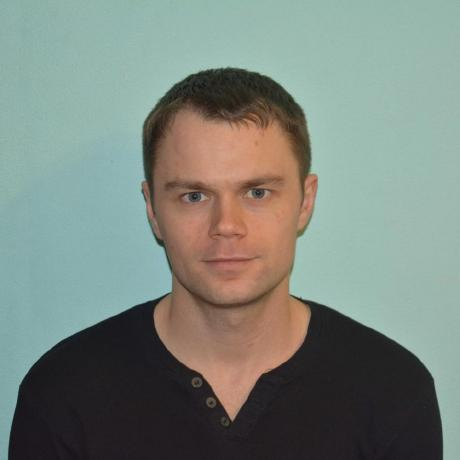
\includegraphics[width=\imagewidth]{photo.jpeg}%
    };
\end{tikzpicture}
%
\section{contacts}
\faMapMarker{} Санкт-Петербург, Россия
~
\faMobilePhone{} +7 (911) 031 7593
~
\faEnvelope{} \href{mailto:iskhomutov@gmail.com}{iskhomutov@gmail.com}
~
\faGithub{} \href{http://github.com/iskhomutov}{iskhomutov}
%
\section{back-end}
Python, Django, Flask, Celery, pytest, fabric, celenium
%
\section{front-end}
ExtJS, BackboneJS, Marionette
%
\section{devops}
Git, PostgreSQL, Heroku
%
\section{misc}
Asterisk, Avaya, Telegram Bot API, 
%
\end{aside}

%----------------------------------------------------------------------------------------
%	SUMMARY SECTION
%----------------------------------------------------------------------------------------
\section{summary}

\begin{itemize}
%----------------------------------------------------------------------------------------
    \item Опыт работы с фреймворками \textbf{Django} и \textbf{Flask};
    \item Опыт в создании UI с применением JS библиотек: \textbf{Marionette}, \textbf{BackboneJS}, \textbf{ExtJS};
    \item Опыт в построении REST/API сервисов с применением \textbf{django-rest-framework} и \textbf{spyne};
    \item Опыт работы с базами данных \textbf{PostgreSQL} и \textbf{SQLite};
    \item Следование \textbf{Agile} методологии при работе над проектом;
    \item Использование консоли как основного инструмента разработки \textbf{NeoVim}, \textbf{virtualenv}, \textbf{psql}.
%----------------------------------------------------------------------------------------
\end{itemize}

%----------------------------------------------------------------------------------------
%	EXPERIENCE SECTION
%----------------------------------------------------------------------------------------
\section{experience}

\begin{entrylist}
%----------------------------------------------------------------------------------------
\entry
  {2017--Now}
  {Fogstream}
  {Хабаровск, Россия}
  {\jobtitle{Full Stack Developer}\\

  Команда разработчиков, основной задачей которых является разработка и сопровождение нескольких государственных проектов 
  (Образование, Сельское хозяйство, Зарплата и Кадры). Все сервисы построены на базе платформы M3, 
  представляющей из себя обертку над Django с интеграцией ExtJS библиотеки в качестве front-end. 
  Демо-версию проекта можно посмотреть по ссылке \href{http://school.bars-open.ru}{school.bars-open.ru}.

  Повседневные обязанности включают:
  \begin{itemize}
      \item Разработка UI с применением \textbf{HTML}, \textbf{CSS}, \textbf{ExtJS}, \textbf{Marionette};
      \item Реализация построителя xls отчетов (\textbf{xlswriter});
      \item Построение веб-сервисов, используя \textbf{spyne} библиотеку;
      \item Оптимизация \textbf{PostgreSQL} запросов;
      \item Рефакторинг legacy кода;
      \item Написание unit тестов;
      \item Описание основного функционала в докстрингах классов/методов;
      \item Использование \textbf{Git} для контроля версий и командной разработки;
      \item Использование инструментов Atlassian (\textbf{Jira/Stash/Confluence}) при разработке проекта;
      \item Ежедневные митинги с участием других разработчиков, аналитиков, тестировщиков.
  \end{itemize}}
%----------------------------------------------------------------------------------------
\entry
  {2013--2017}
  {Sberbank of Russia}
  {Хабаровск, Россия}
  {\jobtitle{VoIP Engineer}\\

  Основные обязанности:
  \begin{itemize}
      \item Администрирование и сопровождение Avaya 5.2 PBX в головном офисе с более чем 3000 пользователями;
      \item Установка, администрирование и сопровождение Avaya IP Office 406/500 PBX в широкой сети ВСП (более 20);
      \item Администрирование Avaya CMS (100 агентов);
      \item Администрирование и настройка Asterisk PBX;
      \item Сопровождение Avaya SES, AES, Contact Recorder;
      \item Сопровождение Cisco CUCM;
      \item Установка и настройка целого ряда оконечных устройств (телефоны, софтфоны);
  \end{itemize}}
%----------------------------------------------------------------------------------------
\end{entrylist}

%----------------------------------------------------------------------------------------
%	EDUCATION SECTION
%----------------------------------------------------------------------------------------
\section{education}

\begin{entrylist}
%----------------------------------------------------------------------------------------
\entry
{2007--2012}
{Диплом по специальности Телекоммуникации}
{Дальневосточный университет путей сообщения (Хабаровск, Россия)}
{\vspace{-0.3cm}}
\end{entrylist}
%----------------------------------------------------------------------------------------
\end{document}
